\documentclass{article}
\linespread{1.5}
\usepackage{graphicx}
\usepackage{amssymb}
\author{Jaime Abbariao \and Nadime Uddin \and Abdul Haque \and Michelle Tam \and Xuming Shi}
\title{MTH 4135 Homework 1}
\date{}
\begin{document}
	\maketitle
	\begin{enumerate}
		\item Download the program \textbf{TimedPi.cpp} and the header files \textbf{Declarations.h} and \textbf{Definitions.h} into the same folder. Compile \textbf{TimedPi.cpp} and run it performing 1 million, 10 million, and 100 million simulations. For each of these runs, attach a screen snapshot.\\\\
		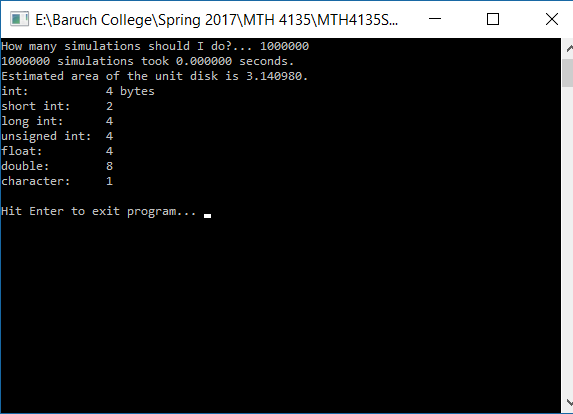
\includegraphics[width=16em]{Homework1_q1_1million.png}
		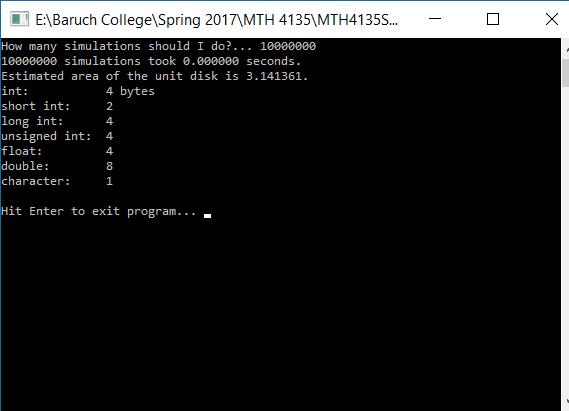
\includegraphics[width=16em]{Homework1_q1_10million.png}
		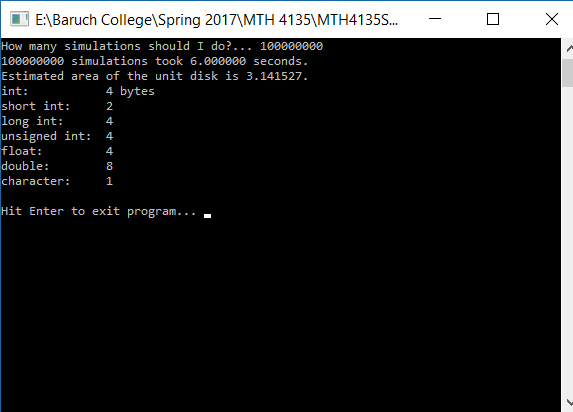
\includegraphics[width=16em]{Homework1_q1_100million.png}
		\item The five dimensional unit ball is the subset of $\mathbb{R}^5$ given by
		$$B = \lbrace (v, w, x, y, z): v^2 + w^2 + x^2 + y^2 + z^2 \leq 1 \rbrace$$
		Let $C$ denote the five dimensional cube $$C = \lbrace (v, w, x, y, z): |v| \leq 1, |w| \leq 1, |x| \leq 1, |y| \leq 1, |z| \leq 1 \rbrace$$
		so $B \subset C$. Since each side of $C$ is of length 2, the five-dimensional "volume" of $C$ is $2^5 = 32$. Modify \textbf{TimedPi.cpp} to use Monte Carlo simulation to estimate what fraction of $C$'s volume is also occupied by $B$. Use this to estimate the five dimensional volume of $B$. You should do at least 100 million simulations. Google the words "n-ball volume" and go to the Wikipedia page. From their formula, compute the numerical value of the volume of the 5 dimensional unit ball.\\
		\textbf{Executive Summary}:\\
		\textbf{Methodology}:\\\\
		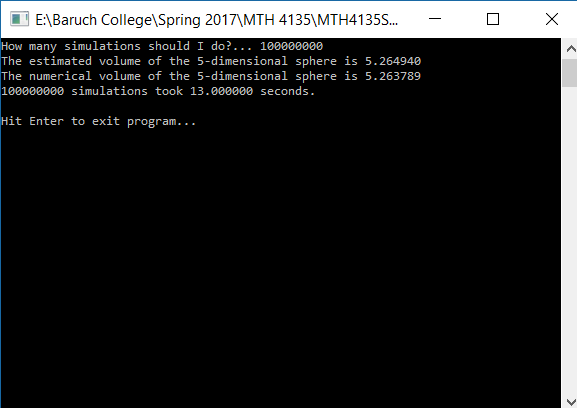
\includegraphics[width=16em]{Homework1_q2_Output.png}
	\end{enumerate}
\end{document}